\chapter{The Large Hadron Collider}
\label{chap:lhc}

The Large Hadron Collider (LHC) is a particle accelerator capable of creating the most energetic (man-made) collisions of particles to date. The LHC is housed within a tunnel 27 km in circumference and 100 m underground, near Geneva, Switzerland. Two beampipes, 5.6 cm in diameter, contain protons circulating in opposite directions around the LHC tunnel. Over 1200 superconducting dipole magnets, 15 m in length and providing a field strength of 8.3 T, are placed along the beamline to guide the protons within the circular trajectory. Radio-frequency electric fields are used to accelerate the particles to nearly the speed of light.

Before the protons are stored in the LHC ring, they must first make their way through a number of stages which comprise the CERN accelerator complex. The protons are sourced from a simple bottle of hydrogen gas. A large electric field is used to ionize the gas and the protons are fed into a linear accelerator (Linac 2) which increases their energy to 50 MeV. These protons subsequently are fed through three synchrotrons: Proton Synchrotron Booster, Proton Synchroton, Super Proton Synchroton, where the proton beam energy is increased to 1.5, 25, and 450 GeV, respectively. After the Super Proton Synchroton, the beamlines of the LHC are filled resulting in two counter-propagating beams of 6.5 TeV each. Figure~\ref{fig:lhc} is a diagram of the entire CERN complex. As can be seen, there accelerator complex is rich with activity. Table~\ref{tab:stages} is a summary of the successive stages relevant in the beam development.

\begin{figure}
\centering
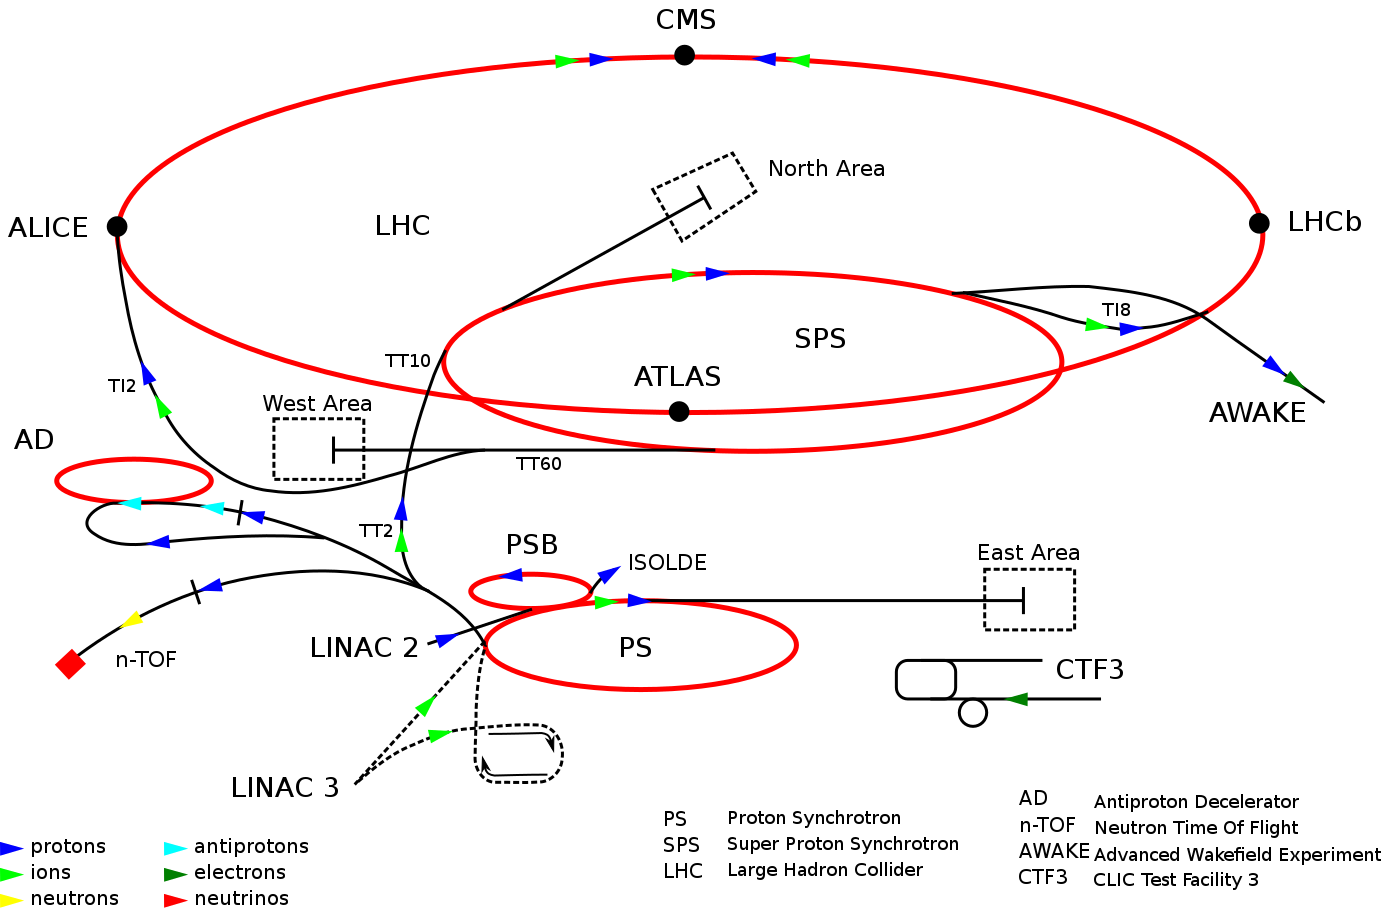
\includegraphics[width=0.7\textwidth]{figs/lhcschematic.png}
\caption{The CERN accelerator complex.}
\label{fig:lhc}
\end{figure}

\begin{table}
\centering
\caption{Successive stages of increasing the proton beam energy.}
\label{tab:stages}
\begin{tabular}{ll}
\hline\hline
stage & final energy\\
\hline
bottle of hydrogen gas & ...\\
Linac 2 & 50 MeV\\
Proton Synchrotron Booster & 1.5 GeV\\
Proton Synchroton & 25 GeV\\
Super Proton Synchroton & 450 GeV\\
LHC & 6.5 TeV\\
\hline
\hline
\end{tabular}
\end{table}

At four points around the ring, magnets are used to further confine and direct each of the two (counter-rotating) beams at one another. At each of these interaction points, there is a large detector placed to capture the remnants of the collisions. These detectors are named CMS, LHCb, ATLAS, and ALICE, and labeled as such in Figure~\ref{fig:lhc}. CMS and ATLAS are considered ``general-purpose'' detectors striving to surround the interaction region as much as possible, allowing to reconstruct a wide variety of particles and the full event. LHCb is specialized for b physics. b hadron production is greatest in the ``forward'' region (parallel to the beampipe) where the LHCb is primarily instrumented; an asymmetrical design where the detector is placed only on one side of the interaction region is. ALICE is specialized for detection of heavy-ion collisions, where the large size of colliding nuclei leads to events with many more particles to reconstruct.

A measure of the rate of particle collisions produced at a collider is given by the \textit{instantaneous luminosity}. It relates the cross section probability ($\sigma$) for some interaction to occur with the expected numbers of events N of those type over some time period: $\textrm{N} = \sigma \int \mathcal{L}(t)$. It is an important parameter of an accelerator as it dictates how many proton interactions can be made within a given amount of time, limiting the total amount of data. In general, the luminosity is dependent on the size and shape of each of the beams, the number of protons in each beam $n_{1,2}$, and how frequently they can be made to interact at the LHC. The instantaneous luminosity can be define as:

\begin{equation}
\label{eq:lumi}
\mathcal{L}(t) = f \frac{n_{1} n_{2}}  { 4 \pi \sigma_{x} \sigma_{y}}
\end{equation}
where f is the collision frequency, and $\sigma_{x}, \sigma_{x}$ are the effective transverse widths of the beams.

In the LHC, the protons within each beam are arranged in 2808 ``bunches'' about 30cm long containing $10^{11}$ protons each ($n_{1}, n_{2}$) (arranged in this manner to the radiofrequency chambers). At each of the interaction points, the bunches are steered into one another every 25 ns ($f=40\,\textrm{MHz}$). Although there are many protons within each bunch, on average there are only about 25 appreciable proton interactions per crossing with a large energy transfer between two partons (constituents of a proton, i.e. quarks and gluons). Each of these interactions creates its own \textit{primary vertex} where many tracks are found to emanate from, indicating a single interaction between two particular protons. The number of additional interactions per bunch crossing is known as \textit{pile up} and poses a formidable challenge in the reconstruction. One of the long term goals for the LHC is to increase its instantaneous luminosity leading to a drastic increase in the number of these vertices which must be reconstructed. In Figure~\ref{fig:pu} we see  the challenge we already face - an image of an event recorded in 2016, the green lines are tracks, the orange dots are interaction vertices.

\begin{figure}
\centering
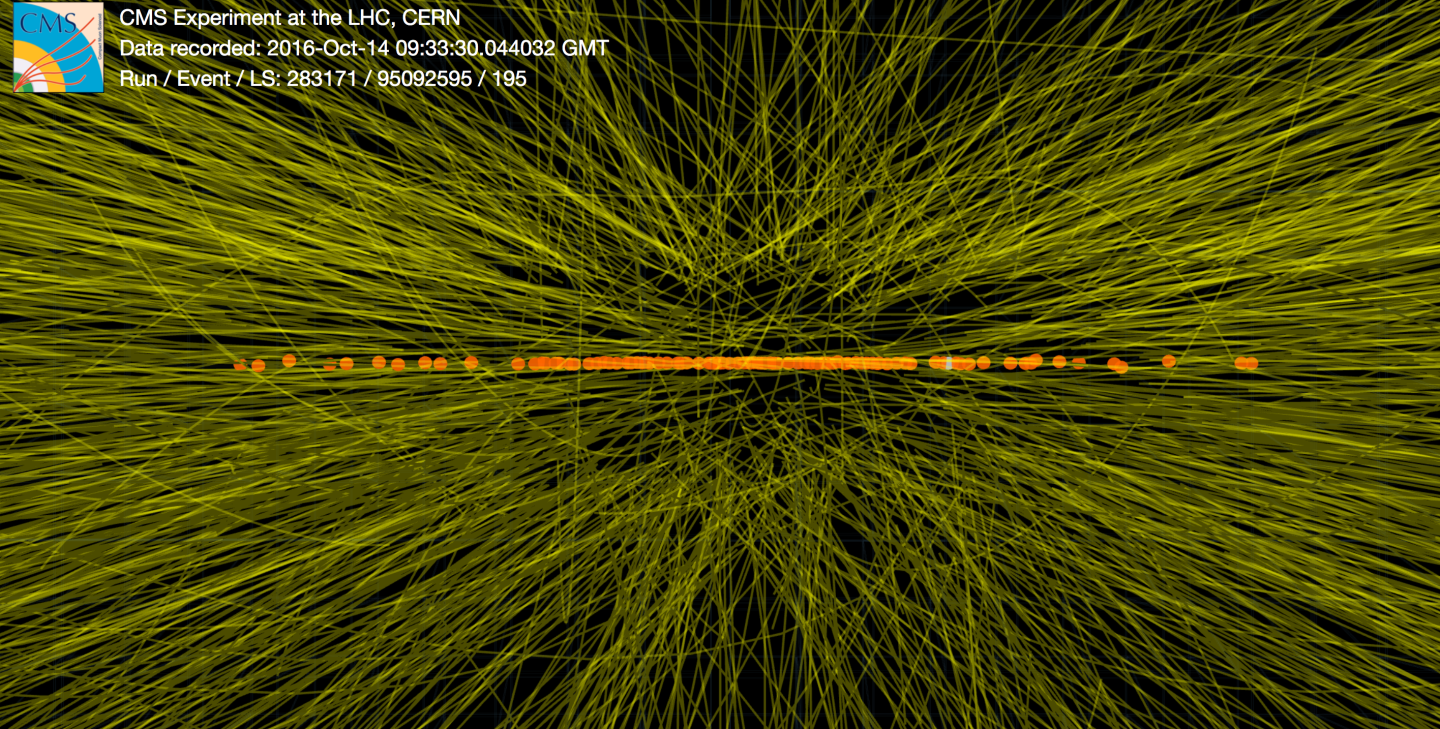
\includegraphics[width=0.5\textwidth]{figs/highpileup0_4.png}
\caption[The number of pileup interactions in a 2016 event recorded by CMS.]{The number of pileup interactions in a 2016 event recorded by CMS \cite{pu}. The green lines are tracks reconstructed in the silicon tracker. The orange dots are identified interaction vertices.}
\label{fig:pu}
\end{figure}

The LHC began taking data in 2009 with a total center-of-mass energy of 900 GeV. The center-of-mass energy of the beam collisions has been increasing over the years, with runs at 7, 8, and now 13 TeV - there is even possibility of extending this to 14 TeV. The high performance of the LHC machine has allowed to take over 150 fb$^{-1}$ in its lifetime, the largest of any experiment to date. Figure~\ref{fig:lumi} shows the integrated luminosity collected by the CMS experiment over this time.

\begin{figure}
\centering
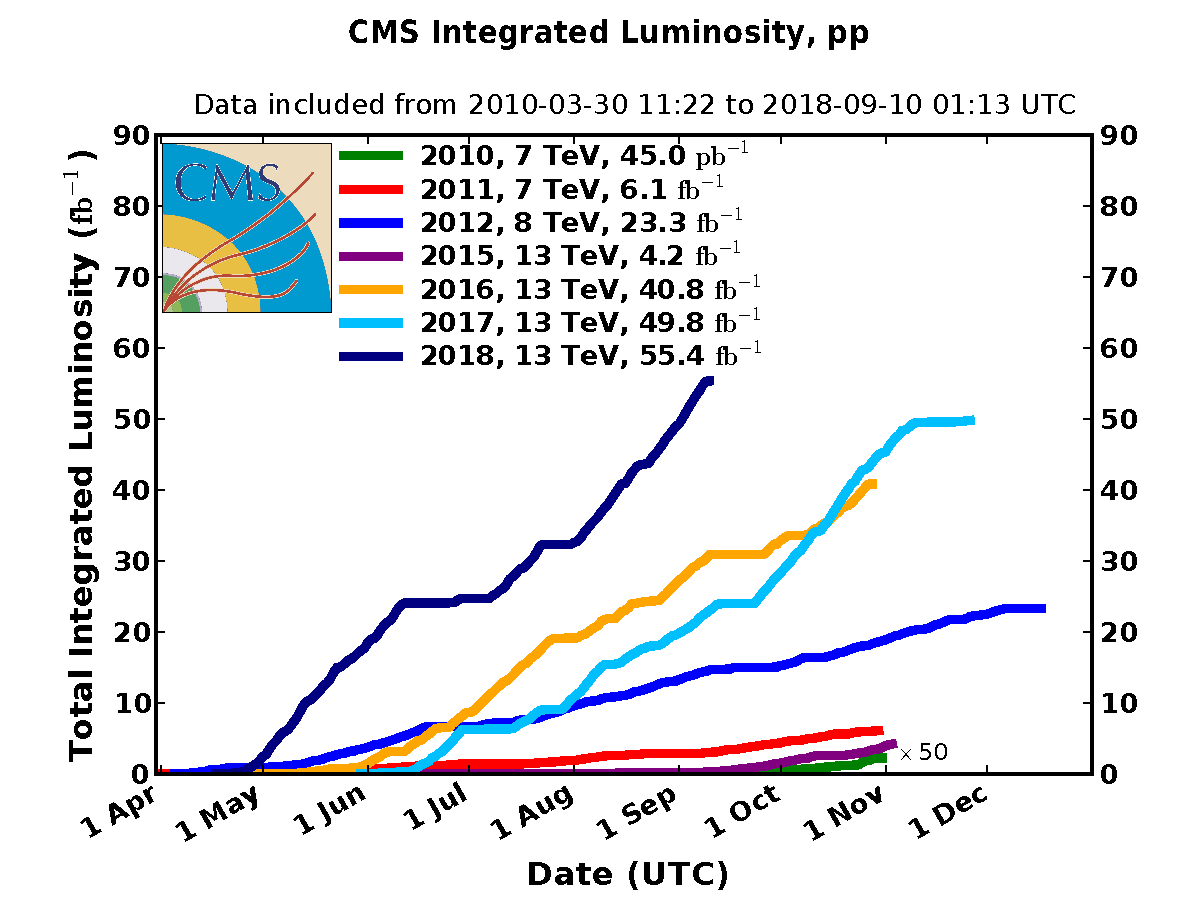
\includegraphics[width=0.5\textwidth]{figs/int_lumi_cumulative_pp_2.pdf}
\caption{The integrated luminosity of CMS over its lifetime.}
\label{fig:lumi}
\end{figure}
